\chapter{Laplace and Inverse Laplace Transform}
Laplace Transform convert a function in time domain into frequency domain in polynomial form. Laplace Transform is used for Analyzing and Solving Ordinary Differential Equation. By using Laplace Transform we can analyze an ODE by just analyze the polynomial equation.
\begin{tcolorbox}[title=Process]
	\begin{center}
		\textbf{Given an Ordinary Differential Equation and Initial Condition}
		\[
		a_2\ddot{x}(t) + a_1\dot{x}(t)+a_0x(t)=b_1\dot{u}(t)+b_0u(t)\quad|\quad x(0) = 0,\dot{x}(0) = 0
		\]
		\[
		\downdownarrows
		\]
		\textbf{Laplace Transform}
		\[
		X(s) = \frac{b_1s+b_0}{a_2s^2+a_1s+a_0} \frac{1}{s}
		\]
		\[
		\downdownarrows
		\]
		\textbf{Partial Fraction Decomposition}
		\[
		X(s) = \frac{k_0}{s}+\frac{k_1}{s+p_1}+\frac{k_2}{s+p_2}
		\]
		\[
		\downdownarrows
		\]
		\textbf{Inverse Laplace Transform}
		\[
		x(t) = k_0 + k_1e^{-p_1t} + k_2e^{-p_2t}
		\]
	\end{center}
\end{tcolorbox}


\section{Laplace Transform}
Definition of Laplace Transform: Given a function in time domain, its Laplace Transform is denoted by:
\[
F(s) = \mathcal{L}\{f(t)\} = \int_{0}^{\infty} f(t)e^{-st} dt
\]
Where : \(s = \sigma + j\omega\)

\subsection{Laplace of Dirac Delta Function}
We have a function :
\[
\delta(t) = \frac{1}{|a|\sqrt{\pi}}e^{-(t/a)^2}
\]
as \(a \rightarrow 0\)
\[
\Delta(s) = 1
\]

\subsection{Laplace of Unit Function}
We have a function :
\[
u(t) = 
\begin{cases}
	1, & \text{if } t\geq 0 \\
	0, & \text{if } t<0     \\
\end{cases}       
\]
We have a Laplace :
\[
U(s) = \int_{0}^{\infty} 1e^{-st} dt = -\frac{1}{s} e^{-st} |_0^\infty = -\frac{1}{s}[e^{-\infty} - e^{0}] = -\frac{1}{s}[0 - 1] = \frac{1}{s}
\]

\subsection{Laplace of $f(t) = e^{-at}$}
We have a function :
\[
f(t) = e^{-at}
\]
We have a Laplace :
\[
\begin{split}
	F(s) &= \int_{0}^{\infty} e^{-at} e^{-st} dt \\
	&= \int_{0}^{\infty} e^{-(s+a)t} dt \\
	&= -\frac{1}{s+a} \int_{0}^{\infty} (-(s+a)t)' e^{-(s+a)t} dt \\
	&= -\frac{1}{s+a} \left[e^{-(s+a)t}\right]_0^\infty  \\
	&= -\frac{1}{s+a} \left[e^{-\infty} - e^0\right]  \\
	F(s) &= \frac{1}{s+a}
\end{split}
\]

\subsection{Laplace of $f(t) = t$}
We have a function :
\[
f(t) = t
\]
We have a Laplace :
\[
F(s) = \int_{0}^{\infty} t e^{-st} dt
\]
Let :
\[
\begin{split}
	u &= t \rightarrow du = dt\\
	dv &= e^{-st} dt \rightarrow v = \int e^{-st}dt = -\frac{1}{s} e^{-st}
\end{split}
\]
\[
\begin{split}
	F(s) &= uv - \int vdu \\
	&= (t) (-\frac{1}{s} e^{-st}) - \int -\frac{1}{s} e^{-st} dt \\
	&= -\frac{t}{s} e^{-st} +\frac{1}{s} \int e^{-st} dt \\
	&= -\frac{t}{s} e^{-st} -\frac{1}{s^2} e^{-st} \\
	&= -(\frac{t}{s} +\frac{1}{s^2}) e^{-st} \\
	&= -\left((\frac{st+1}{s^2}) e^{-st} \right) |_0^\infty \\
	&= \frac{1}{s^2}
\end{split}
\]

\subsection{Laplace of Integral of a Function}
We have an integral of a function:
\[
f(t) = \int_{0}^{t} f(\tau) d\tau
\]
We have a Laplace:
\[
\begin{split}
	F(s) &= \int_{0}^{\infty} (\int_{0}^{t} f(\tau) d\tau) e^{-st} dt \\
	&= \int_{0}^{t} f(\tau) d\tau (-\frac{1}{s}) e^{-st} |_0^\infty + \int_{0}^{\infty} \frac{1}{s} e^{-st} f(t) dt \\
	&= \frac{1}{s} \int_{0}^{\infty} f(t) e^{-st} dt
\end{split}
\]

\subsection{Laplace of Derivative of a Function}
We have an integral of a function:
\[
f(t) = \frac{df(t)}{dt}
\]
We have a Laplace:
\[
\begin{split}
	F(s) &= \int_{0}^{\infty} \frac{df(t)}{dt} e^{-st} dt \\
	&= e^{-st} f(t) |_0^\infty + \int_{0}^{\infty} f(t) se^{-st} dt \\
	&= -f(0) + s \int_{0}^{\infty} f(t) e^{-st} dt
\end{split}
\]
\[
\mathcal{L}\{\frac{df(t)}{dt}\} = s\mathcal{L}\{f(t)\} - f(0)
\]


\subsection{Final Value Theorem}
FVT is used to relate the steady state behavior of \(f(t)\) to the behavior \(sF(s)\). If a function has a Laplace transform, then:
\[
\lim_{t->\infty} f(t) = \lim_{s->0} sF(s)
\]
\paragraph{Example 1} We have a system
\[
\Omega(s) = \frac{K}{s(\tau s + 1)}
\]
To find the steady state value of \(\omega(t)\), we get:
\[
\omega_{ss} = \lim_{s->0} s\frac{K}{s(\tau s + 1)} = K
\]
\paragraph{Example 2} We have a system
\[
\begin{split}
	\dot{\omega}(t) + a \omega (t) &= b u(t) \\
	s\Omega(s) + a\Omega(s) &= b U(s) \\
	\Omega(s)(s+a) &= b U(s) \\
	\Omega(s) &= \frac{b}{(s+a)} U(s)
\end{split}
\]
Case 1 : We want to study when \(u(t)=V_0\) is step function, thus \(U(s) = \frac{V_0}{s}\), we get a system:
\[
\Omega(s) = \frac{V_0b}{s(s+a)}
\]
\begin{itemize}
	\item Check if the poles of the system is on the left-half plane
\end{itemize}
By finding the roots of denominator of the system \(s\Omega(s) = \frac{sV_0b}{s(s+a)} = \frac{V_0b}{(s+a)}\). We see the root is \(s = -a\) where \(a\) is positive, thus the pole of the system in on the left-half place. \\
Finding the steady state of the system:
\[
\omega_{ss} = \lim_{s->0} s\Omega(s) = \lim_{s->0} s\frac{V_0b}{s(s+a)} = \lim_{s->0} \frac{V_0b}{(s+a)} = \frac{V_0b}{a}
\]
Case 2 : We want to study when \(u(t)=t\) is ramp function, thus \(U(s) = \frac{1}{s^2}\), we get a system:
\[
\Omega(s) = \frac{b}{s^2(s+a)}
\]
\begin{itemize}
	\item Check if the poles of the system is on the left-half plane
\end{itemize}
By finding the roots of denominator of the system \(s\Omega(s) = s\frac{b}{s^2(s+a)} = \frac{b}{s(s+a)}\). We see the root is \(s = -a\) and \(s=0\). The root \(s=0\) is exactly on the imaginary axis, thus the pole of the system in not on the left-half place. Thus the system will not come to rest at the final value.




\section{Inverse Laplace Transform}
We want to inverse the Laplace Transform from frequency domain back to time domain.
\[
f(t) = \mathcal{L}^{-1}[F(s)] = \oint_{{\gamma-iT}}^{{\gamma+iT}} e^{st} F(s) ds
\]
From the inverse Laplace Transform from definition, it is very hard. We want to manipulate the Laplace Transform into an easier and recognizable form to easily inverse it. 

\subsection{Case 1: Distinct Real Poles}
\paragraph{Example}
\[
F(s) = \frac{s^2+8s+15}{s^3+3s^2+2s} = \frac{7.5}{s} + \frac{-8}{s+1} + \frac{1.5}{s+2}
\]
\[
\begin{split}
	\mathcal{L}^{-1}[F(s)] &= \mathcal{L}^{-1}[\frac{7.5}{s}] + \mathcal{L}^{-1}[\frac{-8}{s+1}] + \mathcal{L}^{-1}[\frac{1.5}{s+2}] \\
	&= 7.5\mathcal{L}^{-1}[\frac{1}{s}] -8\mathcal{L}^{-1}[\frac{1}{s+1}] + 1.5\mathcal{L}^{-1}[\frac{1}{s+2}] \\
	f(t) &= 7.5.1(t) -8e^{-1t} + 1.5e^{-2t}
\end{split}
\]
\subsection{Case 2: Repeated Real Poles}
\paragraph{Example}
\[
F(s) = \frac{s^2+2s+3}{(s+1)^3} = \frac{1}{s+1} + \frac{2}{(s+1)^3}
\]
\[
\begin{split}
	\mathcal{L}^{-1}[F(s)] &= \mathcal{L}^{-1}[\frac{1}{s+1}] + \mathcal{L}^{-1}[\frac{2}{(s+1)^3}] \\
	&= \mathcal{L}^{-1}[\frac{1}{s+1}] + 2\mathcal{L}^{-1}[\frac{1}{(s+1)^3}] \\
	&= e^{-1t} + 2(\frac{1}{(3-1)!}t^{3-1}e^{-1t}) \\
	f(t) &= e^{-1t} + t^2e^{-t}
\end{split}
\]
\subsection{Case 3: Complex Conjugate Poles}
\paragraph{Example}
\[
F(s) = \frac{s-1}{s^2+2s+2} = \frac{s-1}{(s+1)^2+1^2}
\]
\[
\begin{split}
	\mathcal{L}^{-1}[F(s)] &= \mathcal{L}^{-1}[\frac{s-1}{(s+1)^2+1^2}] = \mathcal{L}^{-1}[\frac{s-1+2-2}{(s+1)^2+1^2}] = \mathcal{L}^{-1}[\frac{s+1-2}{(s+1)^2+1^2}] \\
	&= \mathcal{L}^{-1}[\frac{s+1}{(s+1)^2+1^2}] + \mathcal{L}^{-1}[\frac{-2}{(s+1)^2+1^2}] \\
	f(t) &= e^{-t} cos(t) - 2e^{-t} sin(t)
\end{split}
\]

\section{Poles Location and Time Domain Response}

\begin{figure}
	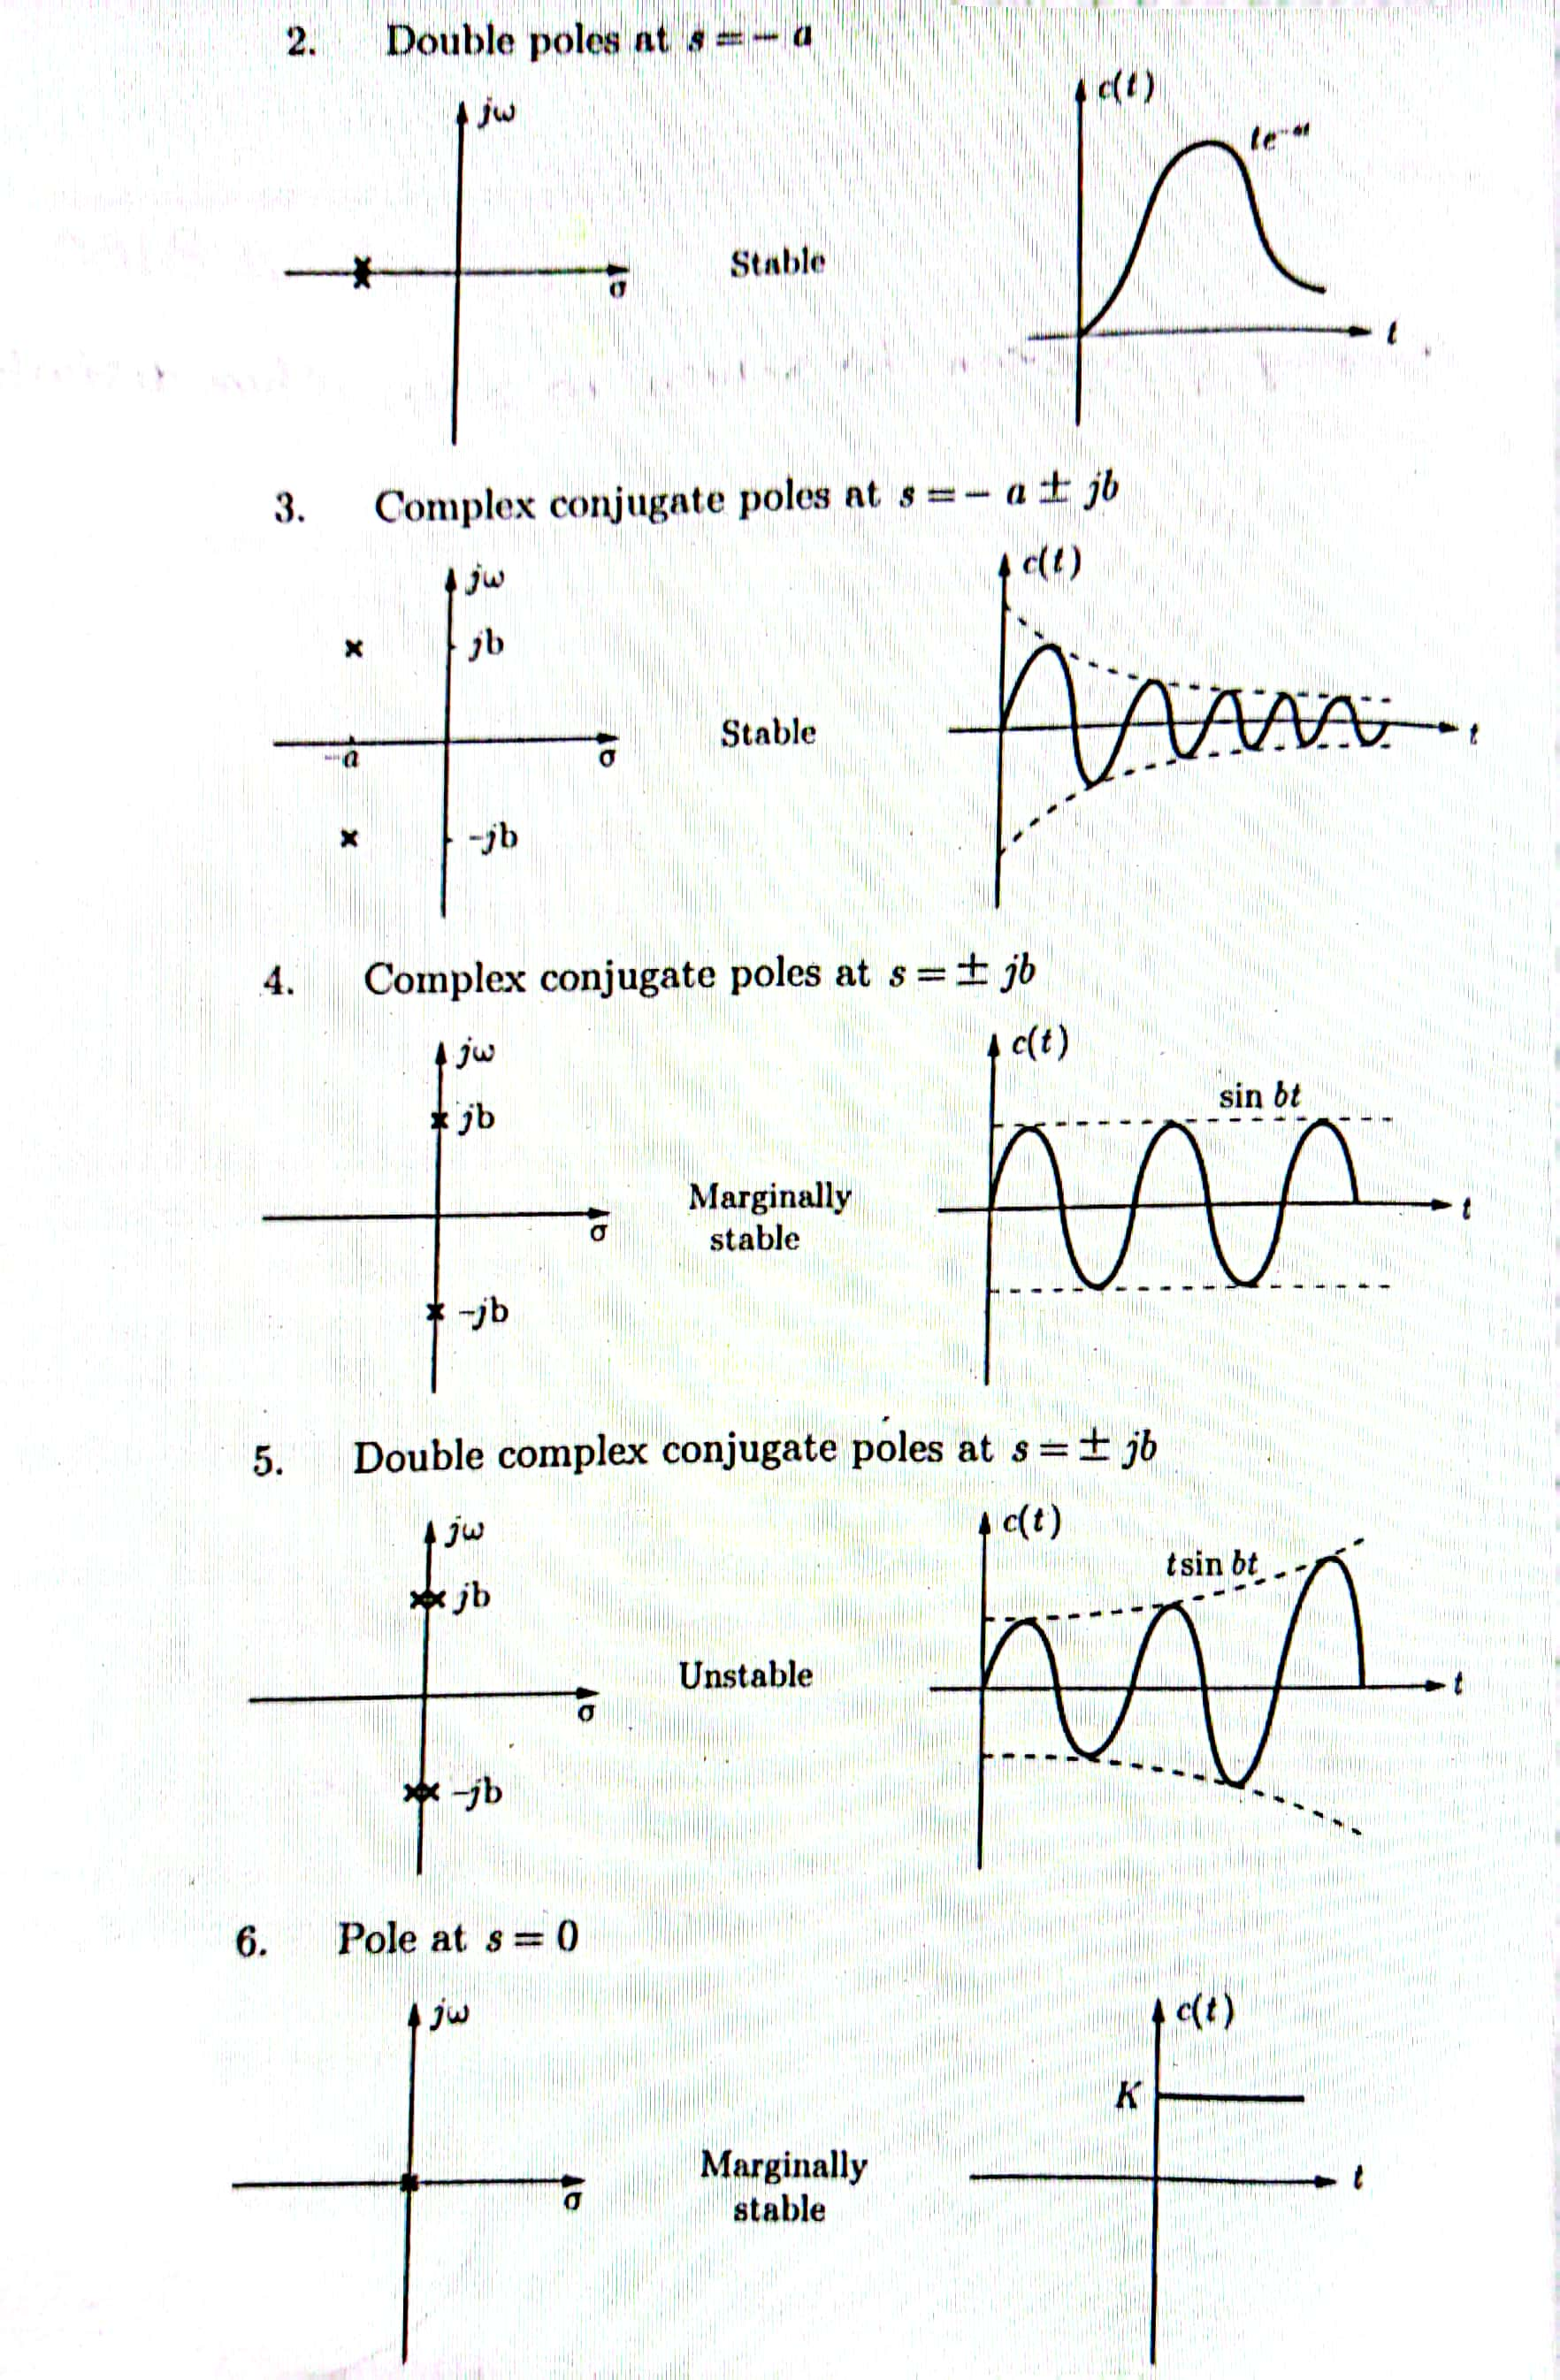
\includegraphics[width=\linewidth]{src/laplace/lpfig1}
\end{figure}
\begin{figure}
	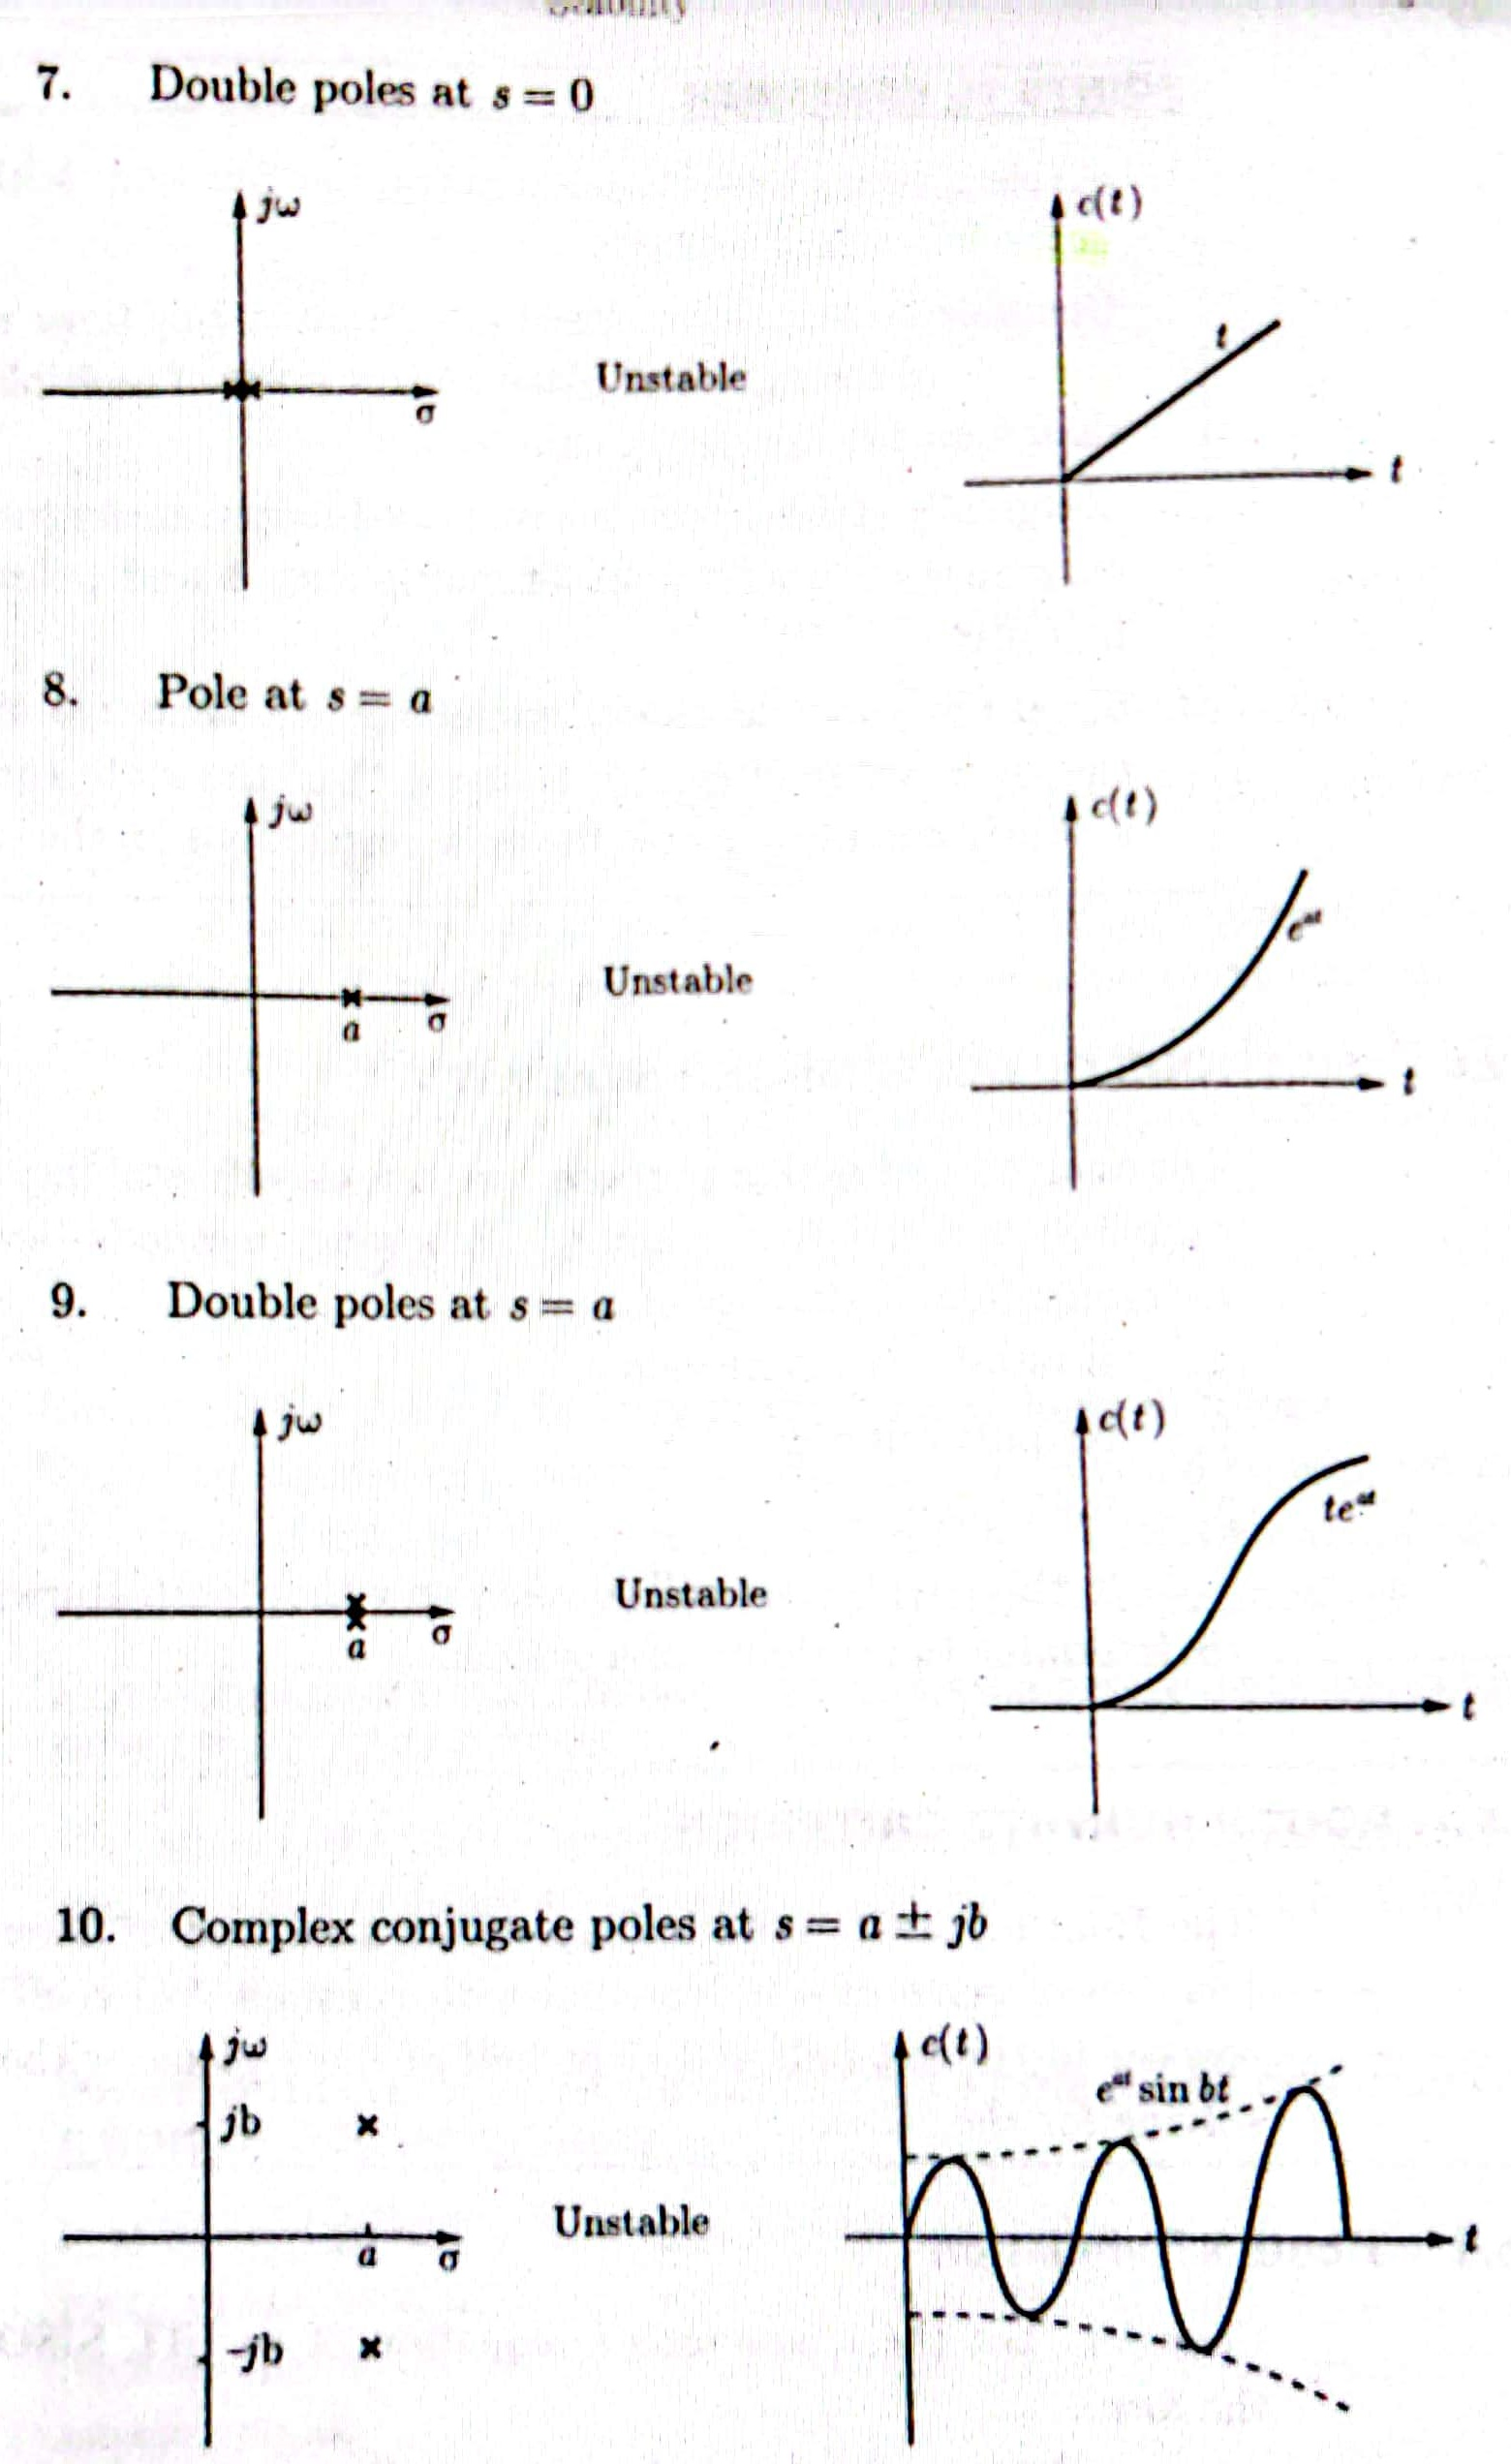
\includegraphics[width=\linewidth]{src/laplace/lpfig2}
\end{figure}
